\documentclass[thesis.tex]{subfiles}
\begin{document}

\chapter{Related Work}
\label{chap:prevwork}

% Categories from GISTAR
% * Finite Elements (also contains voxel based GI)
% * Monte-Carlo ray tracing
% * Photon Mapping
% * Instant Radiosity
% * Many lights (hierarchical! gathering of lights)
% * Point-based (render points somehow)
% * Discrete ordinate methods (propagation volumes etc.)
% * Precomputation

This chapter gives an overview of related realtime global illumination techniques.
Ritschel et al. \cite{bib:RealtimeGIOverview} already gave a great overview over this field for all approaches before 2012.
Therefore, we will focus on newer methods and those which are either fundamental, similar or inspirational to this thesis instead of trying to cover the whole field.

\section {Many-Lights Methods}
\begin{figure}[h]
	\centering
	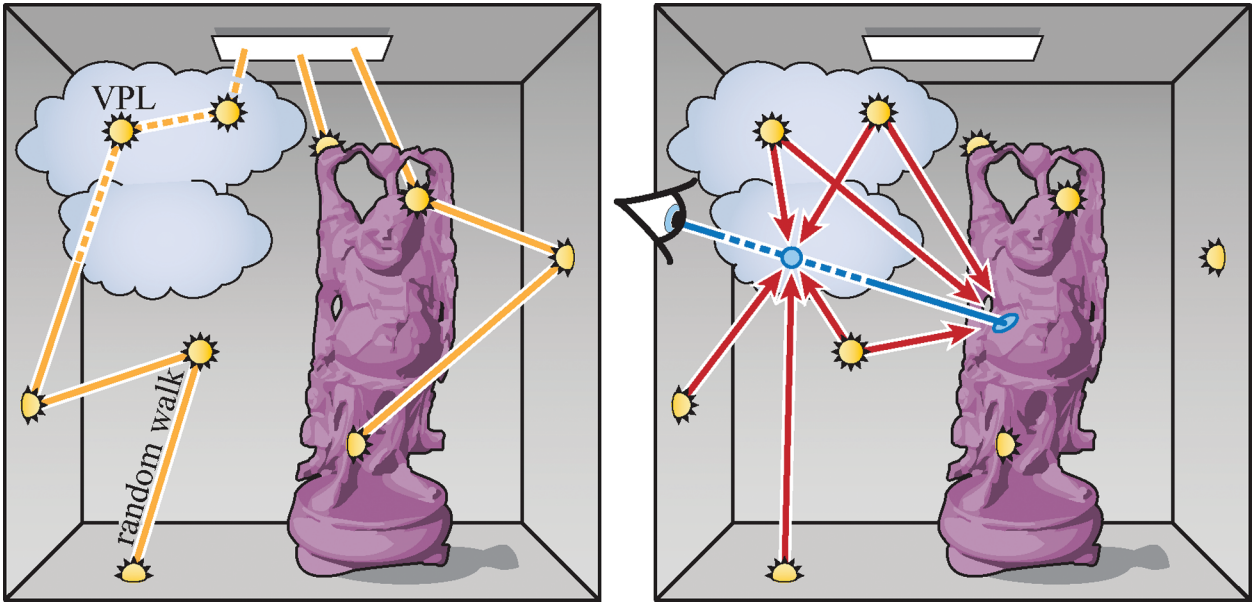
\includegraphics[width=0.8\textwidth]{manylights}
	\caption{\cite{bib:manylightssurvey2014} Two passes of many-light algorithms: Left distribution of virtual lights, right direct lighting using virtual lights.} \label{fig:manylights}
\end{figure}
Many-light methods reduce the global illumination to the smaller problem of calculating the direct lighting of many virtual light sources.
The basic principle was first described in Keller's work on Instant Radiosity \cite{bib:instantradiosity} (IR).
All many-light approaches perform two passes (see \autoref{fig:manylights}):
First virtual light sources are distributed in the scene, second each virtual light source performs direct lighting.
The main advantages of the many-light approach in general is its relatively easy unified framework and its good scalability in performance and quality.
Global illumination using $M$ virtual lights can generally be expressed as following:
\begin{equation}
L_o(\mathrm{x}, \omega_o) = \sum\limits_{i=1}^{M} f_r(\mathrm{x}, \overrightarrow{\mathrm{x}\mathrm{x}_i}, \omega_o) \cdot G(\mathrm{x}, \mathrm{x}_i) \cdot V(\mathrm{x}, \mathrm{x}_i) \cdot f_r(\mathrm{x}_i, \omega_i, \overrightarrow{\mathrm{x}_i\mathrm{x}}) \cdot \phi_i
\end{equation}
Where $G(\mathrm{x}, \mathrm{x}_i)$ is the geometry term which describes the light transfer from the virtual light in $x_i$ to the surface in point $x$.
It depends on the type of the virtual light source.
$V(\mathrm{x}, \mathrm{x}_i)$ is the visibility of a virtual light and $\phi_i$ its incoming flux.
The original IR distributes the light by tracing photon rays from the light source that are bounced inside the scene.
As also many more recent techniques, IR used virtual point light sources (VPL).

Dachsbacher et al. \cite{bib:manylightssurvey2014} did recently a detailed survey on many-lights for both offline and real-time rendering.
We focus here on the most important real-time approaches.

\subsection{Reflective Shadow Mapping}
One of the most important real-time global illumination algorithms is reflective shadow mapping by Dachsbacher et al. \cite{bib:reflectiveshadowmaps} on which many other approaches, including the one presented in this thesis, rely.
It handles the virtual light distribution with the rasterization of an extended shadow map, the reflective shadow map (RSM).
The RSM does not only contain depth as normal shadow maps, but also the reflected flux and the normal of the surface in each texel.
Each texel of this shadow map is then seen as virtual point light.
The original paper shades each pixel with a given number of sampled VPLs without taking indirect shadows into account.
Also, the technique handles only a single indirect bounce of diffuse lighting which means that a VPL is strictly speaking a hemispherical Lambert emitter.
(Like most literature we will use the term "VPL" interchangable)

While RSM offers an easy way to generate virtual lights in real-time generation of, it does basically not alter the way how those lights are applied and how their visibility is determined.
There are a few techniques that try to reduce the number of virtual lights and create few virtual area lights (VAL) by clustering
Both Dong et al. \cite{bib:clusturedvisiblity:dong} and Prutkin et al. \cite{bib:clusturedvisiblity:prutkin} suggest to cluster VPLs using k-means.
The former performs the clustering in world-space, the later directly in image space of the RSM.
Both approaches suffer from temporal coherence problems since the size and position of the clusters can change rapidly.

\subsection{VPL Bias and Compensation}
Using virtual point lights, the geometry term is defined as following:
\begin{align}
G(\mathrm{x}, \mathrm{x}_i) = \frac{(\hat{\mathbf{n}} \cdot \overrightarrow{\mathrm{x}\mathrm{x}_i} )^+}{||\mathrm{x} - \mathrm{x}_i||^2} \cdot (\hat{\mathbf{n}}_i \cdot \overrightarrow{\mathrm{x}_i\mathrm{x}})^+
\end{align}
Where $\mathbf{n}$ and $\mathbf{n}_i$ are the surface normals in point $\mathrm{x}$ and $\mathrm{x}_i$ respectively.
Note that the geometry term is a combination of the photometric distance law (fraction of cosine of angle to light source and squared distance to light source) and the definition of intensity for Lambert emitter (cosine of angle to receiver) as described earlier in \autoref{sec:preq:theo:relation}.
\\
\begin{figure}[h]
\centering
\begin{subfigure}[b]{0.48\textwidth}
	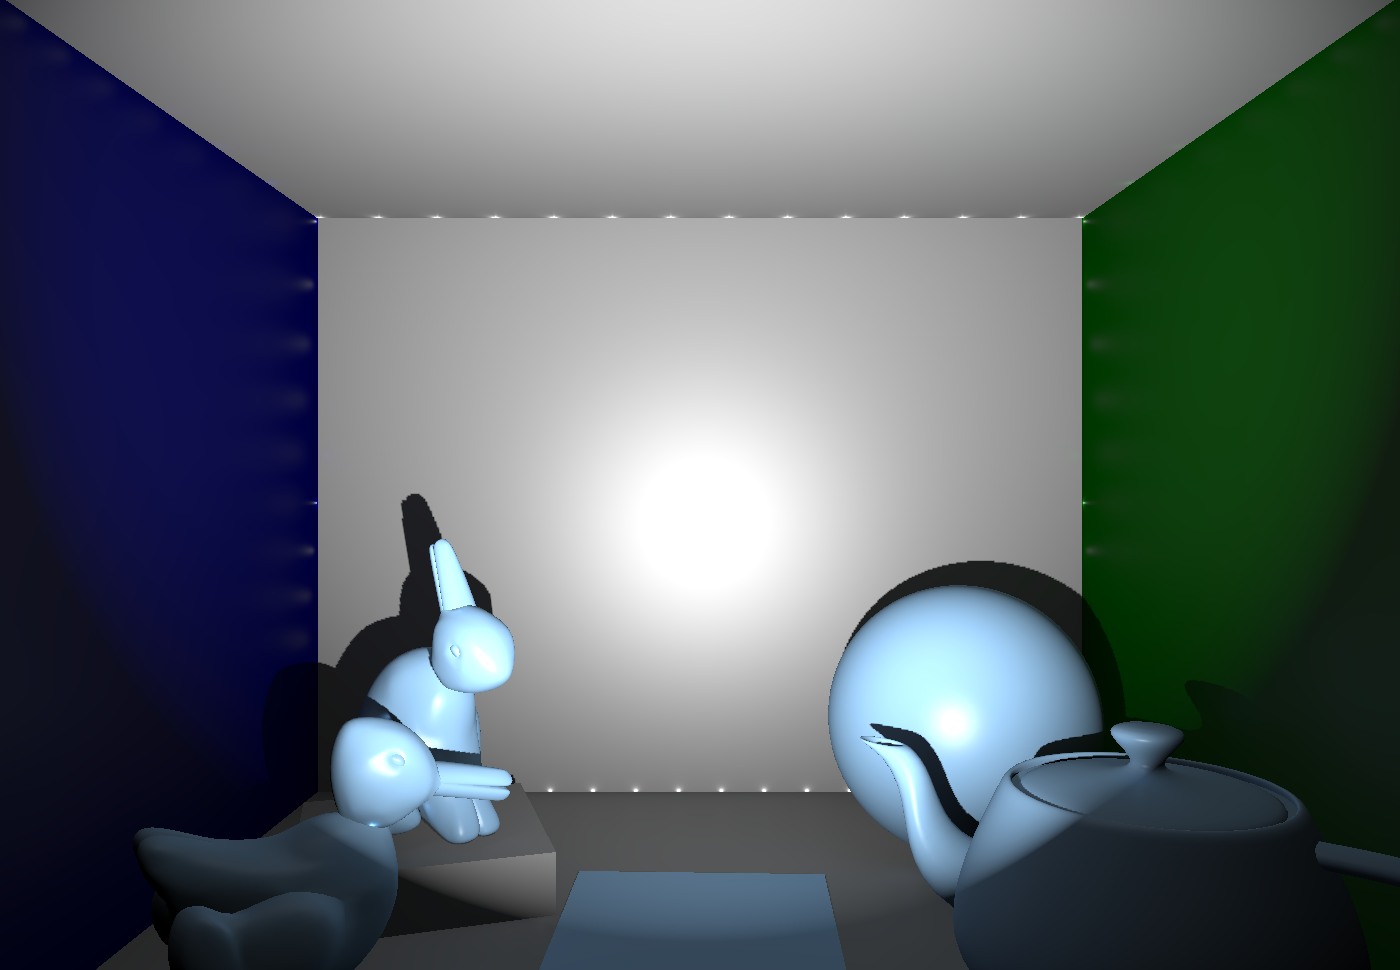
\includegraphics[width=\textwidth]{rsmbias/default}
\end{subfigure}
\begin{subfigure}[b]{0.48\textwidth}
	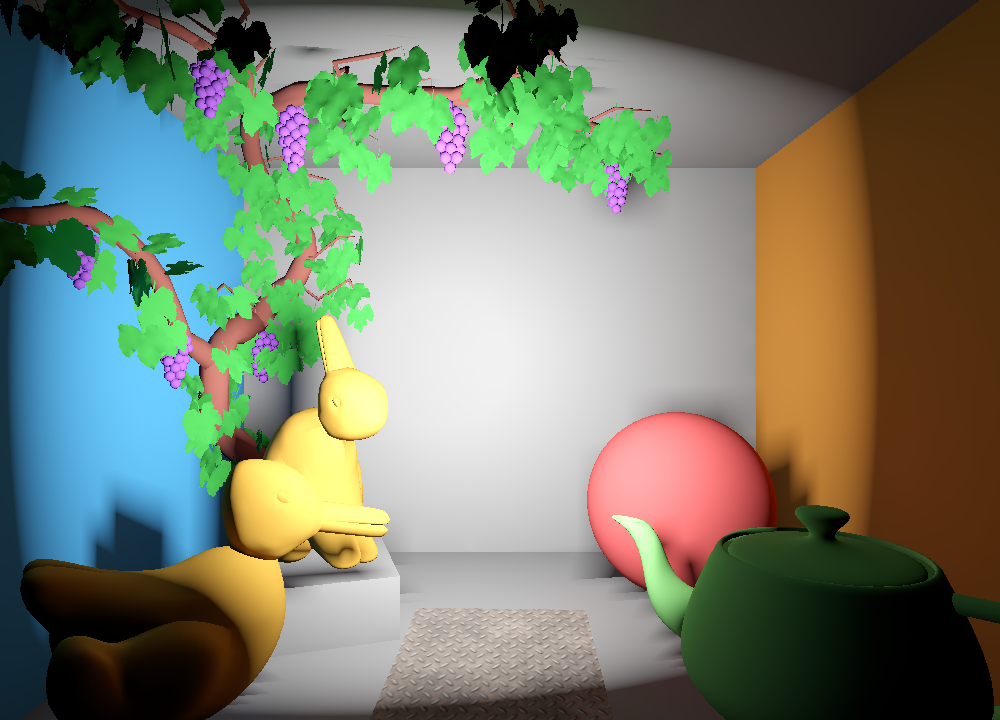
\includegraphics[width=\textwidth]{rsmbias/val}
\end{subfigure}
\caption{Left: Small bright splotches due to inverse squared distance in geometry term. Right: Using virtual area lights as proposed in \cite{bib:LightskinPaper}.}\label{fig:rsmbias}
\end{figure}
The inverse-squared distance between shading point and light source introduces a singularity, as this distance is zero in the limit.
Therefore, the contribution of a VPL reaches infinity in such a point.
The result are bright splotches, mostly visibility in creases, as seen left in \autoref{fig:rsmbias}.

Typically these artifacts are avoided by clamping the geometry term to a user defined maximum which obviously introduces a bias.
There are several bias compensation techniques:
Kollig and Keller \cite{bib:biascomp:kk04} shoot rays to nearby surface and evaluate the lighting there to transport it back to the original surface.
However, this technique may degenerate to path-tracing is thus not suitable for interactive applications.
Other techniques try to compensate the bias approximately.
For example the bias compensation by Nov\'{a}k et al. \cite{bib:biascomp:novak11} stores the bounded transport in screen-space and computes then residual transport.
Although it misses invisible surfaces, it is both efficient and plausible in its results.
\\
There are also several approaches that use different types of virtual light sources instead of VPLs.
Ha{\v{s}}an et al. \cite{bib:biascomp:vsl} introduce a new light type, the virtual spherical light (VSL).
Instead of a point-to-point evaluation, this allows them to integrate over the solid angle subtended by the spherical light sources.
Their approach is biased but does not cause bright splotches and preserves the overall energy by redistributing.
\\
Lensing et al. \cite{bib:LightskinPaper} use approximate disc shaped lights.
Since they use reflective shadow maps, the area of these virtual areal lights $A_{VAL}$ can easily be estimated by the distance of the VAL to the light source and the solid angle a RSM texel subtends.
They show that if all surfaces are assumed to be diffuse, the lighting can be solved analytically by a simple change in the geometry term:
\begin{align}
G(\mathrm{x}, \mathrm{x}_i)_{VAL} = \frac{(\hat{\mathbf{n}} \cdot \overrightarrow{\mathrm{x}\mathrm{x}_i} )^+}{||\mathrm{x} - \mathrm{x}_i||^2 + A_{VAL}} \cdot (\hat{\mathbf{n}}_i \cdot \overrightarrow{\mathrm{x}_i\mathrm{x}})^+
\end{align}
Using this geometry term, splotches at specular surfaces with low roughness can still occur.
However, most singularities are no longer visible (see \autoref{fig:rsmbias} right).
We use this technique in our approach since it is extremely fast, easy to implement and more plausible than a bounded geometry term.

Bias compensation in participating media are considerably more complex but not handled in this thesis.

\subsection{Shadows for Many-Lights}
Computing visibility for a large number of virtual lights is a difficult problem for realtime renderer since classic shadow computations like shadow mapping are far to expensive for this task.
There are a few methods that try to optimize shadow mapping for rendering large amount of lights:
\\
Imperfect shadow maps Ritschel et. al. \cite{bib:imperfectshadowmaps} leverages the fact that exact secondary visibility is not needed.
First points are placed at random locations on the scene geometry.
Shadow maps are then computed using these points instead of triangles which is much faster.
Holes in the shadow maps are filled with a push-pull heuristic.
The succeeding paper \cite{bib:imperfectshadowmaps:adapative} makes the technique (both VPL placement and shadowing) view adaptive and allows larger scenes.
\\
Olsson et al. \cite{bib:virtualshadowmaps} stores shadow maps on a large virtual texture and decides for each frame which lights actually need to compute shadow maps, how high their resolution should be and which objects act as occluders.
All these operations are performed on the GPU.

Other methods like Micro-rendering by Ritschel et al. \cite{bib:microrendering} or ManyLoDs by Holländer et al. \cite{bib:manylods} use hierarchical data structures to be able to render objects at the exactly needed detail.
This allows very fast approximations of visibility.
However, these techniques have also several other implications for example on how shading performed which is why they are often separately categorized as \emph{point-based GI}.

%\subsection{Shading}
%Multi-resolution splatting techniques ([All Nichols] Hierarchical
%image-space radiosity for interactive global illumination, Multiresolution splatting for indirect illumination, Interactive indirect illumination using adaptive multiresolution splatting) are not as efficient as "Tiled Deferred Shading" (according to \cite{bib:clusturedpreconvoledradiancecaching} (where it is just a side note!)) ... logically Tiled Deferred Shading is even better.
%Interleaved Sampling (Interleaved sampling. In
%Proc. of Eurographics Workshop on Rendering (2001)) also a good idea 
%
%Clustured Forward/Deferred Shading: Finding Unique clusturs is DIFFERENT in paper \cite{bib:clusturedshading} and practical implementation like "Pratical Clustured Shading" (SIGG2013, Humus). Paper uses (local) sorting and page tables. Humus uses Volume Texture. Ollson Siggra2013 presentation uses parallel prefix sum.
%

\section{Caching Methods}
Many recent real-time global illumination methods, including our own, compute indirect lighting only for special \emph{light caches} and interpolate the results of those across many pixels.
Which quantities a light cache saves varies from technique to technique as well as the strategies that is responsible for creating light caches either at runtime or as a pre-computation step.
Since our approach relies on dynamic cache placement, its implications and trade-offs will be discussed in \autoref{sec:impl:dyncacheplace}.
Since caches are mostly placed relatively sparse, most of the following techniques are prone to light bleeding artifacts, i.e. light "seeping" incorrectly through blockers.

\subsection{(Irr-)Radiance Caching}
The basic idea of light caches was first introduced by Ward et al. \cite{bib:irradiancecaching} in the form of Irradiance Caching (IC) to speed up path-tracing.
Each time a ray intersects a diffuse surface it first checks if there are nearby caches from which the irradiance can be interpolated, if not, the irradiance is computed and a new cache is created at this place.
There are many extensions to this method, most notably Radiance Caching by Krivanek et al. \cite{bib:radiancecaching} (RC) which supports arbitrary glossy surfaces by saving incoming radiance encoded in a high order spherical harmonics representation.

\begin{figure}[h]
	\centering
	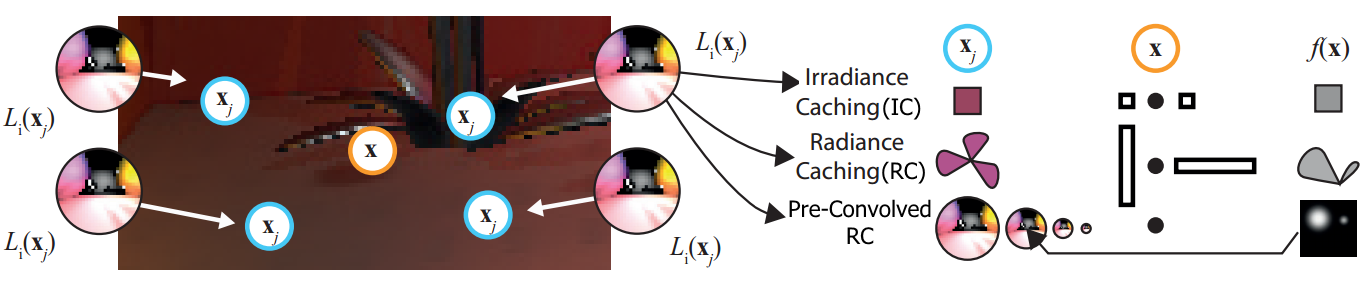
\includegraphics[width=\textwidth]{preconvolvedradiancecaching}
	\caption{\cite{bib:preconvoledradiancecaching} Storage and evaluation of pre-convolved RC in comparison with "classic" IC/RC.
	IC store a single value,
	RC store a series of SH components,
	pre-convolved RC store mipmaps of incoming radiance.} \label{fig:preconvolvedradiancecaching}
\end{figure}
Pre-convoled Radiance Caching by Scherzer et al. \cite{bib:preconvoledradiancecaching} is able to perform radiance caching with a single indirect bounce at interactive frame-rates.
As in the original radiance caching, caches lie on surface.
Each cache renders a hemisphere of all incoming radiance values as depicted in \autoref{fig:preconvolvedradiancecaching}.
The result is then pre-convolved using mipmapping to be able to evaluate quickly arbitrary specular exponents (the paper makes use of the Phong BRDF).
Caches are placed statically and apply their results using splatting, i.e. rendering them directly to a deferred shading buffer.
Clustured Pre-Convolved Radiance Caching, an extension to the previous method by Rehfeld et al. \cite{bib:clusteredpreconvoledradiancecaching}, places the radiance caches according to screen-space clusters which makes the technique more scalable but less temporal coherent.
Additionally it uses cone tracing (which will be explained in \autoref{sec:prev:voxelmethods}) in a prefiltered voxel instead of rasterization to render the cache's radiance hemispheres.

\subsection{(Irr-)Radiance Volumes}

\begin{figure}[h]
	\centering
	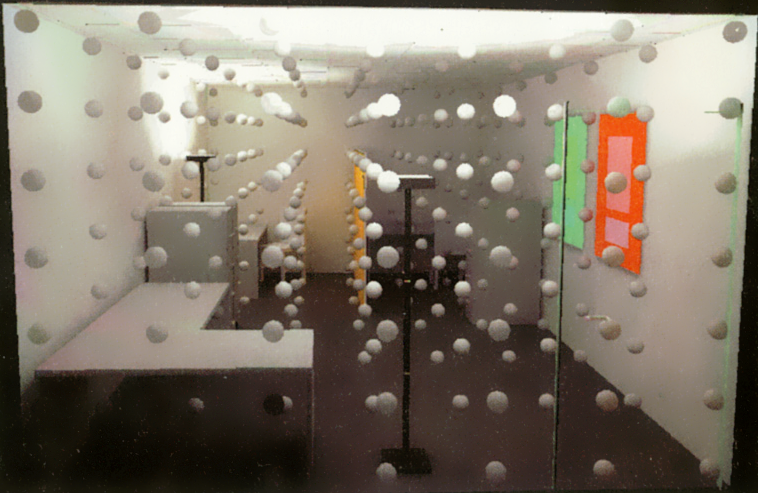
\includegraphics[width=0.7\textwidth]{gregerirradiancevolume}
	\caption{\cite{bib:irradiancevolume} Visualization of an irradiance volume. Each sphere visualizes a light cache colored by the local irradiance for each direction. } \label{fig:irradiancevolume}
\end{figure}
Irradiance volumes as proposed by Greger et al. \cite{bib:irradiancevolume} are very popular to light dynamic objects in otherwise static environments.
An irradiance volume is a regular grid in which each grid cell saves precomputed irradiance values for all directions.
The original work uses hemispherical grid mappings to save irradiance values.
However, other representation like spherical harmonics are common in praxis.
Objects to be lit can then use their normal vectors to look-up the precomputed irradiance values to perform diffuse lighting.
Note however that this method can does not handle light bounced off or occluded by dynamic objects.

The advantage of saving irradiance for all possible normals over saving incoming radiance for each direction, is that an irradiance signal has a much lower frequency than radiance.
Only a single irradiance value is needed for diffuse lighting of a surface (i.e. a given normal) which is equivalent to a hemispherical integration over the incoming radiance.
Nonetheless, if arbitrary BRDFs are to be supported, the total incoming irradiance for a given normal is not sufficient and integration over radiance is necessary.
Note however, that for a spherical harmonics representations, integration over a lobe given in SH has the same costs as evaluating the SH coefficients for a certain direction (as earlier described in \autoref{sec:preq:shprojectrecon}).

\subsubsection{Real-Time}
Njasure et al. \cite{bib:nijasure:rtirradiancevol} compute radiance volumes at runtime with interactive frame rates by rendering a cubemap at each grid point and compute a low number of spherical harmonics coefficients from each of them.

Radiance Hints by Papaioannou \cite{bib:radiancehints} retrieve radiance from a RSM and approximate multiple diffuse light-bounces between the light caches.
Like the RSM algorithm on which the technique is based, occlusion of VPLs is not handled.
For the secondary bounces however, visibility of the radiance hints (= light caches) is approximated by the minimum and maximum distance of the used RSM samples.
\\
Vardis et al. \cite{bib:radiancecachechromaticcompression} improve recently upon Radiance Hints by using chrominance compression and an optimized radiance cache positioning.
Using less SH bands for the chroma part of the radiance allows higher order for the more importance luminance portion.
Which radiance caches that contribute to the scene's surfaces is determined by down-sampling a real-time voxelization.
Contrary to Radiance Hints, caches in mid-air will not be updated.
A dilated version of this volume can be used to determine the visibility of virtual light sources.


\section{LightSkin}
 % % % % % % % % % % % % % % % % % % % % % % % % % % % % % % % % % % % % % % % % % % % % % % %
\begin{figure}[h]
\centering
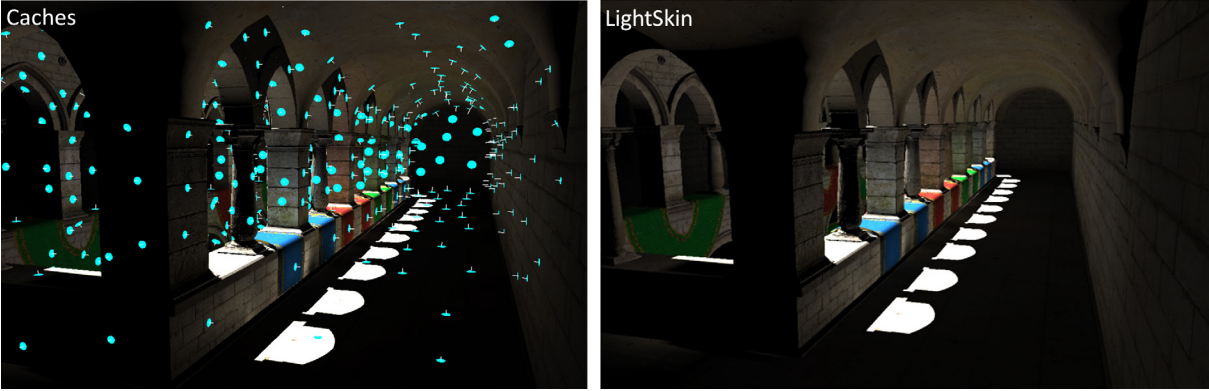
\includegraphics[width=\textwidth]{lightskin}
\caption{\cite{bib:lightskinthesis} LightSkin indirect lighting approach.\\
Left: Cache distribution. Right: Lighting results. } \label{fig:lightskin}
\end{figure}
% % % % % % % % % % % % % % % % % % % % % % % % % % % % % % % % % % % % % % % % % % % % % % % %
LightSkin \cite{bib:LightskinPaper} by Lensing et al. uses precomputed light cache positions which are placed directly on surfaces (see \autoref{fig:lightskin}).
This has several advantages over radiance volume approaches.
Each cache computes the lighting only for a single given normal and set of material properties.
The technique exploits pre-computed neighbor-relation ships for an efficient real-time interpolation of both indirect diffuse and glossy reflections which is dependent on the current lighting situation.
A smooth indirect shadow approximation is achieved by adding a precomputed size to the light caches which makes it possible to use them as coarse blocker.
The combination of clever cache placement during the pre-computation and the sophisticated interpolation at runtime, makes it possible to achieve a relatively high lighting quality even for low amounts of caches, without any temporal artifacts.

While an expensive pre-computation step is needed to place the light caches, compute their neighbors and determine their properties, the approach is not limited to static scenes as caches can be moved with animated objects.
Depending on the number of caches only smooth lighting can be performed and the technique does not scale well with large scenes, since the number of caches for distant objects can not be reduced trivially.
Neighborship-relations are either saved per vertex or on a texture. 
Both methods can increase the memory footprint of a scene considerably.

Furthermore, Lensing describes in his PhD thesis \cite{bib:lightskinthesis} how to use LightSkin for subsurface scattering effects and proposes how to use the method in mixed reality scenarios.

\section{Discrete Ordinate Methods}
Discrete ordinate methods compute light transport by exchanging energy between a cellular discretization of the scene.
Usually it is possible to update the lighting iteratively across many frames.
As long as there are no high frequency changes, slow adaption can exploit frame coherencies to benefit the overall performance drastically.

% % % % % % % % % % % % % % % % % % % % % % % % % % % % % % % % % % % % % % % % % % % % % % % %
\begin{figure}[h]
\centering
\begin{subfigure}[b]{0.35\textwidth}
\centering
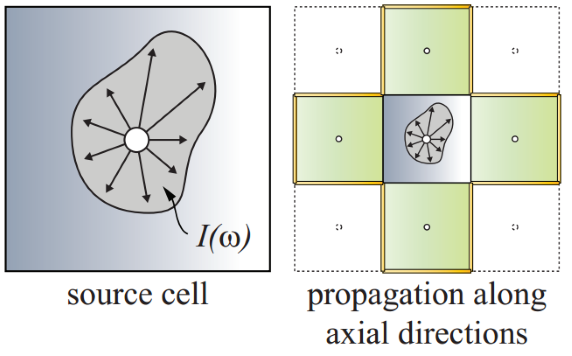
\includegraphics[width=\textwidth]{lpv/principle}
\caption{Light propagation principle.}
\label{fig:lpv:principle}
\end{subfigure}
\begin{subfigure}[b]{0.53\textwidth}
\centering
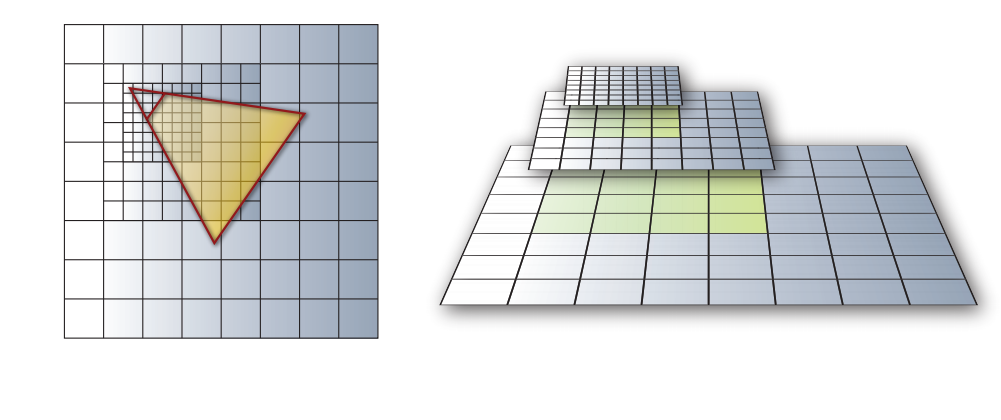
\includegraphics[width=\textwidth]{lpv/cascading}
\caption{Cascading of multiple LPVs.}
\label{fig:lpv:cascading}
\end{subfigure}
\\
\begin{subfigure}[b]{0.48\textwidth}
\centering
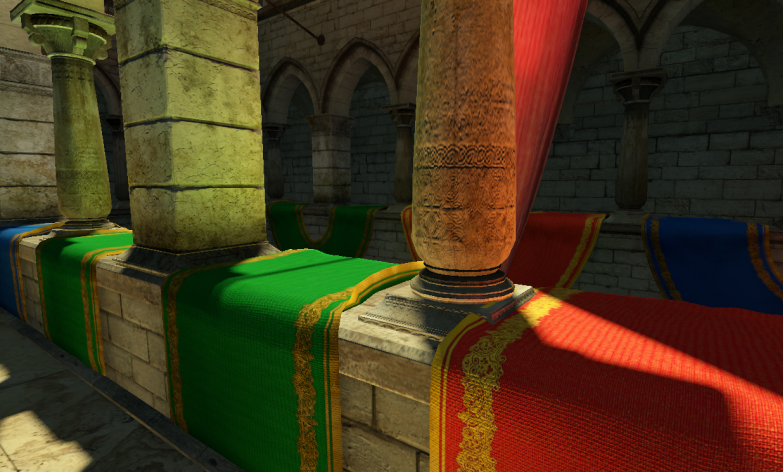
\includegraphics[width=\textwidth]{lpv/lowfreq}
\caption{Low frequency indirect lighting.}
\label{fig:lpv:results}
\end{subfigure}
\begin{subfigure}[b]{0.48\textwidth}
\centering
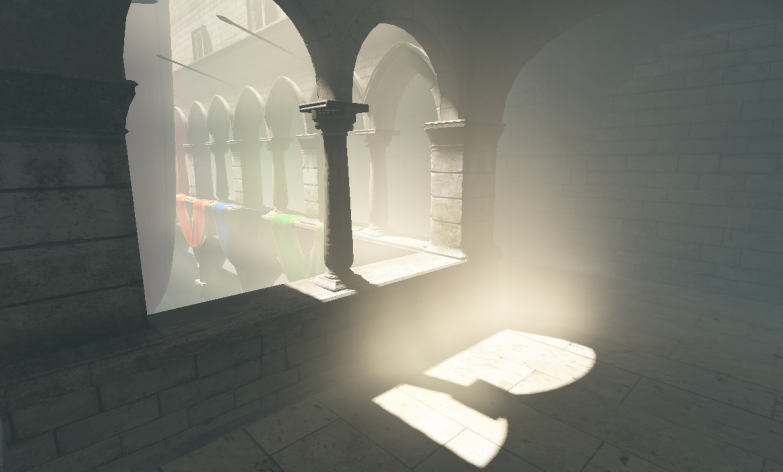
\includegraphics[width=\textwidth]{lpv/media}
\caption{Lit participating media.}
\end{subfigure}
\caption{\cite{bib:lpt} Cascaded LPV, principles and results.}
\end{figure}
% % % % % % % % % % % % % % % % % % % % % % % % % % % % % % % % % % % % % % % % % % % % % % % %
A popular real-time representative of these methods is Cascaded Light Propagation Volumes by Kaplanyan and Dachsbacher \cite{bib:lpt}.
Using a RSM, light is injected into a light propagation volume (LPV).
The LPV is a regular grid where each cell contains a light intensity distribution represented by a few low order spherical harmonic coefficients.
A second grid stores a volumetric representation used for fuzzy occlusion.
Considering these blockers, the light is then propagated across the LPV in each frame (see \autoref{fig:lpv:principle}).
For better scalability with larger scenes, multiple nested LPVs are used as visualized in \autoref{fig:lpv:cascading}.
After the propagation, the LPVs can easily be used to light the scene.
The approach does not rely on any pre-computation and is able to capture both diffuse and low frequency specular lighting in real-time (see \autoref{fig:lpv:results}).
However, it is very prone to light bleeding artifacts and depending on the LPV resolution light may only be transported for rather short distances.
\\
The original approach obtained the blocker volume from the already existing information in RMS and the camera view.
Rasterized Voxel-based GI by Doghramachi \cite{bib:rasterizedvbgi} presents an alternative real-time voxelization approach alongside with several implementation improvements.

\todo{more discrete ordinate methods or rename section}

\section{Voxel-Volume Methods} \label{sec:prev:voxelmethods}
Due to the increasing processing power of GPUs and the development of real-time voxelization algorithms, methods using ray or cone tracing within a voxelized scene representation have gained popularity in the last few years.
Voxelized representations have several advantages over classic triangle-based scenes:
The level of detail can be scaled, random access using world coordinates can easily achieved, intersections tests are simple to perform etc..
The simplest data structures contain only a single binary value per voxel, weather it is solid or not (binary voxelization).
However, it is easy to encode other informations like flux, normals or continuous opacity as well.

\subsection{Voxelization via Rasterization}
The GPUs rasterization capabilities can be used for extremly fast voxelization.
There are boundary voxelizations that encode only the surfaces of an object and solid voxelizations which also capture the interiors of a model as well.
Solid voxelization is generally more difficult to achieve since more writes are needed.
Also the interior of an object might not always be clearly defined.

A general problem with GPU rasterization is the lack of conservativity. 
For voxelization it is usually needed that all voxels that are touched by a triangle are marked.
This is already not the case for standard 2D rasterization.
\cite{bib:GPUGems2}[Chapter 42] by Hasselgren et al. propose to enlarge triangles and and remove potentially unused pixels again discarded in the fragment shader to overcome this issue.
Very recent GPUs expose new rasterization modes to accomplish conservative rasterization more quickly in hardware \cite{bib:nvconservativeraster}.

%Since GPU rasterization rules are There are various algorithms with different 

One of the first algorithms using the GPUs rasterization pipeline was invented by Fang and Chen \cite{bib:fangvoxelization} which needed to draw the entire scene once per volume slice.
A later approach by Dong et al. \cite{bib:dong:voxelization} Eisemann and D{\'e}coret \cite{bib:eisemann:boundaryvox} achieve binary voxelization in a single pass.
Since it writes to one or more 2D targets it achieves a limited bit depth and can not write directly to a volume texture.
The algorithm was later extended to support solid geometry as well \cite{bib:eisemann:solidvox}. 
\cite{bib:dong:voxelization} presented a similar approach that handles geometry that lies parallel to the viewing direction better. 

% % % % % % % % % % % % % % % % % % % % % % % % % % % % % % % % % % % % % % % % % % % % % % %
\begin{figure}[h]
\centering
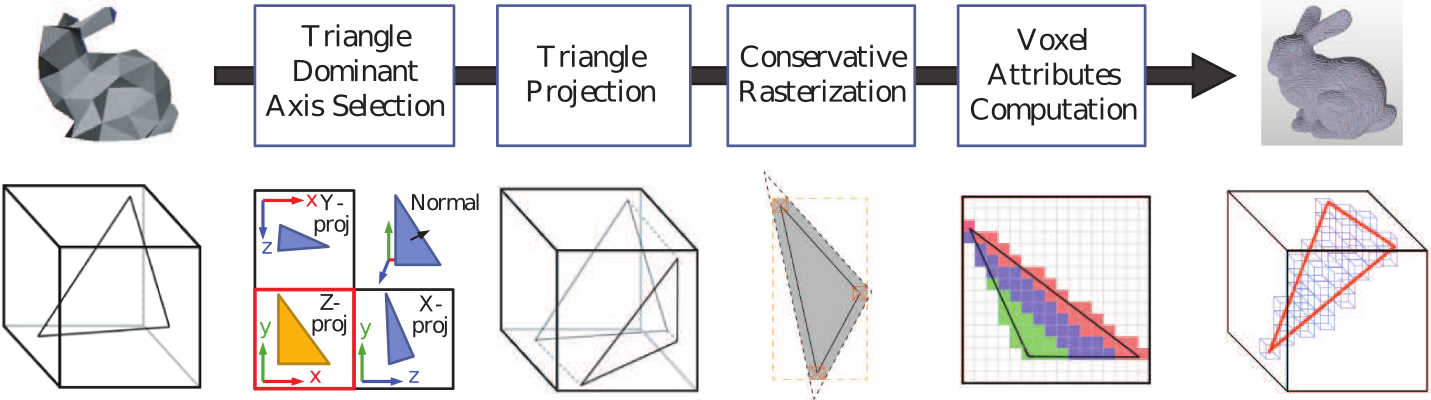
\includegraphics[width=\textwidth]{voxelizationpipe}
\caption{\cite{bib:openglinsightsvoxel} Illustration of single pass voxelization pipeline. }
\label{fig:voxelization}
\end{figure}
% % % % % % % % % % % % % % % % % % % % % % % % % % % % % % % % % % % % % % % % % % % % % % % %
Many of the previous methods relied on graphics hardware which was not able to perform random write accesses.
Newer methods leverage these possibilities and are able to perform high quality boundary voxelization in a single pass.
In this thesis we rely on a conservative single pass voxelization technique by Crassin and Green \cite{bib:openglinsightsvoxel}.
\autoref{fig:voxelization} illustrates how it works.
The geometry shader decides for each triangle its dominant direction and uses it as projection axis to maximize the output of the rasterization stage.
Conservative rasterization, is achieved with the earlier mentioned technique by Hasselgren et al. \cite{bib:GPUGems2}[Chapter 42]. 
Each pixel writes up to three values along the projection axis into the volume texture to mark all voxels that are touched by the source triangle.
If necessary additional attributes can be computed in the fragment shader.

\subsection{Voxel Cone/Ray Tracing}
Voxel-Based GI by Thiedemann et al. \cite{bib:voxelgi} traces multiple rays at each seen world position through a binary voxelization.
When the rays hit a surface or exceed a maximum stepping length, light is added to the ray starting point using a RSM if the hit point lit succeeds the shadow mapping test, i.e. is visible by the light source.
Since tracing rays through the voxel-volume is a very costly operation, indirect lighting remains only local.

 % % % % % % % % % % % % % % % % % % % % % % % % % % % % % % % % % % % % % % % % % % % % % % %
\begin{figure}[h]
\centering
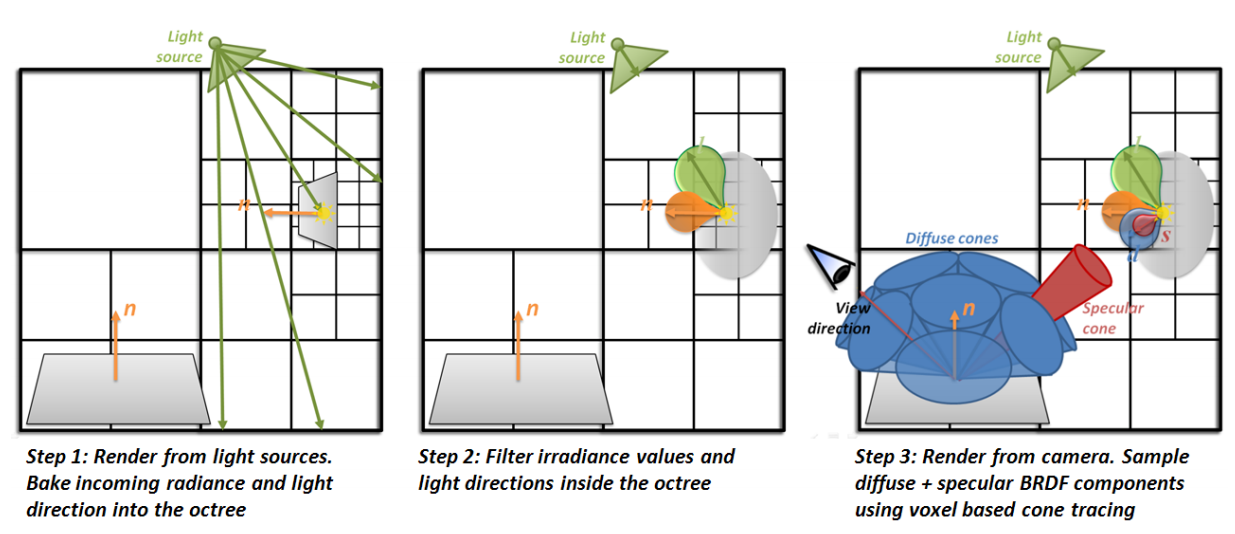
\includegraphics[width=\textwidth]{voxelconetracing}
\caption{\cite{bib:voxelconetracing} Illustration of Voxel Cone Tracing. } \label{fig:voxelconetracing}
\end{figure}
% % % % % % % % % % % % % % % % % % % % % % % % % % % % % % % % % % % % % % % % % % % % % % % %
Voxel Cone Tracing by Crassin et al. \cite{bib:voxelconetracing} overcomes this issue by tracing cones instead of rays through a mip-mapped voxel volume.
Additionally to the occlusion value, each voxel also saves a normal and flux which was before injected by an RSM.
\autoref{fig:voxelconetracing} gives a short overview over the approach.
For diffuse lighting a few cones covering the hemisphere are traced in each visible point.
The step size during the tracing increases together with the sampled mipmap of the voxel volume, so that the entire cone is sampled approximately.
This technique allows Voxel Cone Tracing to trace very long cones at relatively low costs.
Since occlusion is fuzzy in all but the lowest mipmap-level, lighting is applied continuously with each sample  depending on its opacity.
The tracing stops when the total until the cone is completely blocked using an emission-absorbed model.
Additionally, each voxel saves its flux anisotropically for more accurate lighting even with higher mip-levels.
Using an extra, thinner cone for the specular highlight the approach achieves relatively accurate reflections within the same framework.
The main draw-back of Voxel Cone Tracing is its high memory footprint.
Because of this the original work makes use of a sparse voxel octree.
However, for practical considerations the technique has been used in production with cascaded volumes instead. \todo{citation needed}

Layered Reflective Shadow Maps by Sugihara et al. \cite{bib:layeredrsm} works very similar but decouples occlusion from lighting data again.
Visibility determination is handled via cone tracing as before while the actual lighting is performed by lookups in a pre-filtered Layered Reflective Shadow Map.
The RSM is split up into multiple layers to be able to create pre-filterable textures without large depth or normal discontinuities.
Doing so avoids most of the memory and initialization/update overhead associated with the large voxel data structure, since each voxel encodes only binary visibility information.
While the approach has a significantly lower memory footprint than the original Voxel Cone Tracing, it suffers from temporal coherency for highly gloss surfaces and does not scale well with the number of light sources.

\section{Summary} \todo{better title? more like "setting into context"?}
There are only few techniques that fulfill the goals of this thesis (\autoref{bib:goals}).
Most notably Voxel Cone Tracing \cite{bib:voxelgi} (VCT) and Cascaded Light Propagation Volumes \cite{bib:lpt} (LPV) are able to perform global illumination without any pre-computations.
Both have already been used in production environements. \todo{citation needed}
VCT achieves very high quality rendering however due to the price of large complicated memory structures (sparse voxel octree on GPU) and compared to LPV at lower framerates.
LPV on the other hand is often not able to catch indirect lighting over longer distances and is very prone to light bleeding artifacts.

Both methods rely on reflective shadow mapping which is fundamental to many real-time lighting approaches.
On the other hand, direct usage of RSMs often suffers from temporal artifacts as seen in many previous works.
Caching light at specific locations leverages the low frequency of most indirect lighting situations and can reduce shading costs tremendously.
Voxelized scene representations are used in many recent works since real-time voxelization is by now cheaply available.

This thesis is mostly inspired by LightSkin \cite{bib:LightskinPaper} which is able to robustly compute both diffuse and indirect lighting at a relatively high quality.
The final algorithm presented in the next chapter is similar to the recent radiance volume method of Vardis et al. \cite{bib:radiancecachechromaticcompression} of which we were not aware until shortly before the end of our project.
However, there are several key differences that will be elaborated in \autoref{sec:eva:comparisiontoother}.


\subfilebib % Makes bibliography available when compiling as subfile
\end{document}